\chapter{Planificació}

En aquest capítol es mostrarà la planificació que es va realitzar en el moment en què el projecte era
només una idea, i es mostraran els canvis que es varen haver de fer fins a arribar a la planificació que ha 
acabat sent. \\

En un primer moment, la planificació del projecte va ser la següent: \\
\\
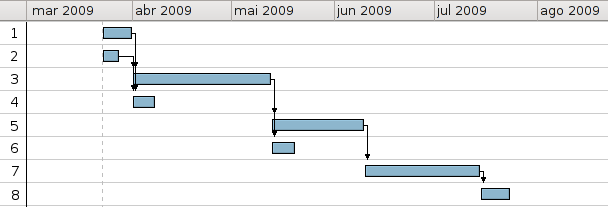
\includegraphics[scale=0.75,keepaspectratio]{primer_gantt2.png} 

\begin{enumerate}
    \item Estructura i disseny del rootkit
    \item Estructura de la documentació
    \item Implementació de les funcionalitats bàsiques
    \item Documentació de les funcionalitats bàsiques
    \item Implementació de les funcionalitats avançades 
    \item Documentació de les funcionalitats avançades 
    \item Injecció de codi en memòria de kernel
    \item Anàlisi general
\end{enumerate}

En aquesta planificació es pot veure que intentem no deixar la documentació del projecte pel final, 
sinó que fos un punt que s'anés avançant constantment. Varem separar les diferents tasques entre: el disseny
i la recerca inicial, la implementació de les funcionalitats (dividides en dos blocs segons la seva dificultat),
una part del rootkit a nivell de kernel per a GNU/Linux, i finalment un anàlisis general per a polir-ho
i homogeneïtzar-ho tot. \\

Sabíem que la recerca tenia un paper molt important en el projecte i que això podia provocar alguns canvis en quant a
les funcionalitats decidides inicialment, i així ha estat.

Sobre aquesta planificació va haver-hi principalment els següents canvis:

\begin{itemize}
    \item Eliminació de la injecció de codi en memòria de kernel (Es va eliminar ja que en kernels actuals ja no 
        és factible, i per tant es va decidir potenciar altres punts. Tot i això s'ha documentat el què i el perquè).
    \item Falta de previsió ja que inicialmet no es varen tenir en compte els períodes d'examens finals i de 
		vacances.
	\item Necessitat de molt més testeig.
\end{itemize}

Com a comentaris importants, dir que la planificació inicial es va veure força afectada a partir de la tercera setmana de Juny, que al apropar-se
examens i entregues finals d'altres assignatures, es va pactar amb el tutor per a fer una petita pausa. \\

L'altre motiu pel qual s'ha acabat allargant una mica més, ha estat la necessitat de dedicar moltes més hores per a 
deixar el rootkit amb l'estabilitat de funcionament desitjada. Totes aquestes funcionalitats programades a tant 
baix nivell (utilitzant llenguatge ensamblador en varis casos) han hagut de ser molt testejades i millorades per a
acabar obtenint un producte de qualitat. \\

Un cop aplicats els diferents canvis que han afectat el projecte, la planificació final ha estat la següent: \\
\\
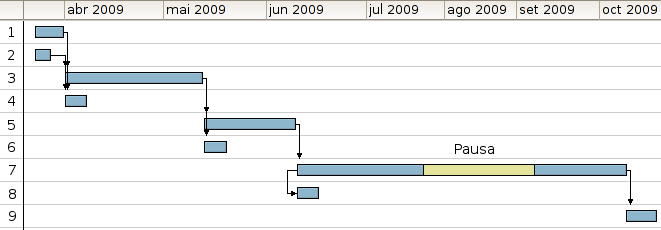
\includegraphics[scale=0.68,keepaspectratio]{segon_gantt.png} 

\begin{enumerate}
    \item Estructura i disseny del rootkit
    \item Estructura de la documentació
    \item Implementació de les funcionalitats bàsiques
    \item Documentació de les funcionalitats bàsiques
    \item Implementació de les funcionalitats avançades I
    \item Documentació de les funcionalitats avançades I
    \item Implementació de les funcionalitats avançades II
    \item Documentació de les funcionalitats avançades II
    \item Anàlisi general
\end{enumerate}

